\documentclass{article}
\usepackage[utf8]{inputenc}

\title{PC Project Report}
\author{Liron Mizrahi, Daniel da Silva}
\date{October 2016}

\usepackage{natbib}
\usepackage{graphicx}
\usepackage{algorithm2e}
\usepackage{subcaption}
\usepackage{amssymb}

\setlength{\parindent}{0em}
\setlength{\parskip}{1em}
\begin{document}

\maketitle


\newpage
\section{Introduction}
K-means is  one of the simplest unsupervised learning algorithms to solve a clustering problem. Clustering is the process of partitioning a group of data points into a small number of clusters. In general, a cluster is defined as a set of similar objects. The similarity in a given set may vary according to data, therefore a clustering algorithm that finds an optimization in one set of data may not find an optimization in another set of data.

There are many variations of the k-means clustering algorithm, however we have looked at 2 of them, namely the normal k-means clustering and online k-means clustering.


\section{Terminology and definitions}
For this report we will define some terms and variables which will be used:
\begin{itemize}
	\item There is a dataset $S \in R^m$.
	\item $\underline{x}$ is a data point in $S$.
	\item $k$ is the number of clusters.
	\item $\underline{\mu_j}$ is a cluster centre.
	\item $d(\underline{x}, \underline{\mu_j})$ is the distance from $\underline{x}$ to $\underline{\mu_j}$.
	\item $N_j$ is the number of points in cluster $j$.
	\item The sum of squared error is given by:
    $$\sum_{j=1}^{k}\sum_{\underline{x} \in S} d(\underline{x}, \underline{\mu_j})^2 $$
	\item $\eta$ is the learning rate where $\eta \in \big[0, 1\big]$. The learning rate is used for the online k-means. It is used to increase or decrease the shift of the centres for each iteration.
\end{itemize}


\newpage
\section{Background Theory}
As stated, k-means is a solution technique to solve a clustering problem. Clustering is the task of grouping a set of objects in such a way that objects in the same group have more similarities to each other than to those in other groups. Clustering is not just one specific algorithm, but it is a problem to be solved. The idea of a cluster cannot be precisely defined, as such different variations of the solution can be derived depending on the idea used of what constitutes a cluster and the method used to find them. This is one of the reasons why there are so many different clustering algorithms. Different cluster models are used by different people depending on their needs, and for each of these cluster models again different algorithms can be given. The cluster model used by k-means is called a centroid model, where each cluster is represented by a single mean vector.

\section{The Clustering Problem}
In centroid clustering, clusters are represented by a vector, which may not necessarily be a member of the dataset. When the number of clusters is fixed to $k$, k-means clustering becomes an optimization problem,i.e. find the $k$ cluster centers and assign the points to the nearest cluster center, such that the squared distances from the cluster are minimized, i.e. the sum squared error (SSE) is minimized. This problem is known to be NP-Hard.


\newpage
\section{k-means vs Online k-means}
K-means and online k-means are very similar in that they accomplish the same task. However, there are some big differences. K-means loops through all the data given and updates the centres after every point has been assigned to their respective closest centre. Each data point can be looked at individually as calculations for the closest centre for each point are not dependent on other points. Each centre is also independent of each other after the points have been assigned to them. This implies that k-means can benefit highly from parallelization. Chunks of data points as well as cluster centres can be processed concurrently.

On the other hand, online k-means is used to deal with continuous streams of data, unlike k-means where all the data is known beforehand. Online k-means looks at one data point at a time and finds the closest centre. Once the centre is found, it is then updated immediately. The problem with this is that calculations are now dependent on prior calculations. As seen above in the online k-means algorithm, the learning rate, $\eta$, is decreased after each iteration, meaning that the calculations for the centres will change depending on the order the data is given. Therefore online k-means is not suitable at all for parallelization.


\section{Theoretical Analysis}
The computational complexity of finding the optimal solution to the k-means clustering problem is known to be NP-hard for a general number of clusters $k$ (even for 2 clusters) and as such a heuristic algorithm must be used such as Lloyd's k-means algorithm shown above. The running time of Lloyd's algorithm is often given as $O(nkmi)$, where $n$ is the number of vectors in $\mathbb{R}^m$ space, $k$ the number of clusters and $i$ the number of iterations needed until convergence.

This complexity analysis lends itself to the decomposition of different aspects of parallelization seen below in section 8.1.
\begin{itemize}
	\item \emph{n} - Datapoints aspect
	\item \emph{k} - Clusters aspect
	\item \emph{m} - Dimensions aspect
\end{itemize}


\emph{Note that i is not relevant to our testing as parallelization cannot improve the number of iterations needed for convergence. (as discussed in section 8.2)}


\newpage


\section{Serial Algorithms}
Shown below is the general pseudo-code for the serial k-means clustering algorithm and the serial Online k-means clustering algorithm:

\begin{algorithm}[H]
\SetAlgoLined
 Given dataset $S$ in $\mathbb{R}^m$\;
 Choose $k$, which is number of clusters\;
 Choose the $k$ cluster centres(Randomly): $\underline{\mu_1}, \underline{\mu_2}, \dots, \underline{\mu_k}$\;
 \While{stopping condition does not hold}{
  \For{each $\underline{x} \in S$}{
    Find $min\big\{d(\underline{x}, \underline{\mu_1}), d(\underline{x}, \underline{\mu_2}), \dots, d(\underline{x}, \underline{\mu_k})\big\}$\;
    Say $d(\underline{x}, \underline{\mu_j})$ is the minimum\;
    Assign $\underline{x}$ to cluster $j$\;
  }
  
  \For{each cluster centre $\underline{\mu_j}$ }{
    move cluster centre to the mean of the points in its cluster\;
    $$\underline{\mu_j} \leftarrow \frac{1}{N_j} \sum_{\underline{x}}{\underline{x}} $$
    where $N_j$ is the number of points in cluster $j$.
  }
 }
 \caption{k-means clustering algorithm (This heuristic algorithm is also known as Lloyd's k-means algorithm}
\end{algorithm}

\begin{algorithm}[H]
\SetAlgoLined
 Given dataset $S$ in $\mathbb{R}^m$\;
 Choose $k$, which is number of clusters\;
 Choose the $k$ cluster centres(Randomly): $\underline{\mu_1}, \underline{\mu_2}, \dots, \underline{\mu_k}$\;
 \While{stopping condition does not hold}{
  \For{each $\underline{x} \in S$}{
    Find $min\big\{d(\underline{x}, \underline{\mu_1}), d(\underline{x}, \underline{\mu_2}), \dots, d(\underline{x}, \underline{\mu_k})\big\}$\;
    Say $d(\underline{x}, \underline{\mu_j})$ is the minimum\;
    Update $\underline{\mu_j}$\;
    $$\underline{\mu_j} \leftarrow \underline{\mu_j} + \eta(\underline{x} - \underline{\mu_j})$$
    where $\eta$ is the learning rate.
  }
  Decrease $\eta$ (This is an extra stopping condition).
  
 }
 \caption{Online k-means clustering algorithm}
\end{algorithm}

The stopping conditions may vary by time or by iterations. However, we have chosen the stopping condition to be bounded by the number of iterations.

\begin{figure}
    \begin{subfigure}{0.5\textwidth}
        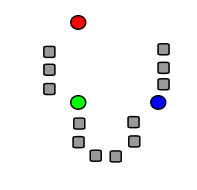
\includegraphics[width=0.9\linewidth, height=5cm]{Pictures/K_Means_Example_Step_1.png}
        \caption{ $k$ initial centres are randomly\\ generated (in this case k=3).}
    \end{subfigure}
    \begin{subfigure}{0.5\textwidth}
        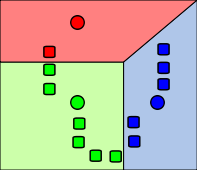
\includegraphics[width=0.9\linewidth, height=5cm]{Pictures/K_Means_Example_Step_2.png}
        \caption{ $k$ clusters are created by associating every data point with the nearest centre.}
    \end{subfigure}
    \begin{subfigure}{0.5\textwidth}
        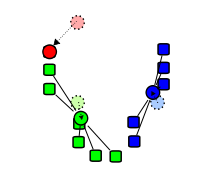
\includegraphics[width=0.9\linewidth, height=5cm]{Pictures/K_Means_Example_Step_3.png}
        \caption{The centre of each of the $k$ clusters\\ becomes the new mean of the points.}
    \end{subfigure}
    \begin{subfigure}{0.5\textwidth}
        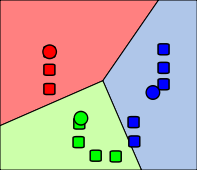
\includegraphics[width=0.9\linewidth, height=5cm]{Pictures/K_Means_Example_Step_4.png}
        \caption{Steps (b) and (c) are repeated until convergence has been reached.}
    \end{subfigure}
\caption{Example demonstrating how k-means works}

\end{figure}



\section{Parallelization of k-means}
\subsection{Three Aspects for Consideration}
The k-means algorithm has multiple ways it can be parallelized. Specifically we look at the following three aspects:
\begin{itemize}
	\item Iterations over datapoints
	\item Iterations over clusters
	\item Iterations over dimensions
\end{itemize}


Important to note is that parallelizing an aspect provides better scalability of that aspect. This means that as the number of one of the above aspects is increased, the speedup from parallelization will improve.

Datapoints is probably the most important area to parallelize efficiently. The whole concept of k-means is clustering multiple points and analysing the clusters. This implies that there are \emph{many} points that need to be classified, hence scalability in this aspect is important as it is exhibits a high proportion of the work done in the algorithm.

In the example of clusters, many clusters may be used although the number of clusters is generally subject to the amount of datapoints (for example, it wold be pointless to have 100 clusters working on 100 datapoint). Hence the number of datapoints can be assumed to still be more important and higher than the clusters.

Our group has decided to exclude the dimensions aspect for now, as to test well we would have to iterate up to around 10 dimensions, and we would of course have to have a respectable amount of points to get an accurate depiction. Furthermore, the iterations over dimensions the operations are generally somewhat limited to simple things such as addition. This means the overhead would be more likely to outweigh the gains for a long time, potentially up to more dimensions than can be reasonably tested.

The code was parallelized in both the datapoints aspect, and the clusters aspect. This provides scalability for both aspects but may slow down the algorithm running on say, 5000 datapoints but only 1 cluster. This is due to the overhead of parallelizing for a single cluster 'wasting' some of the speedup.

It is important to note that not all these aspects have equal footing when considering the sheer volume of the input for each. It is also important to examine the work done per iteration on a particular aspect. For example, iteration over datapoints is one of the more costly operations as for each datapoint, distances to each cluster must be calculated and the minimum of these distances must also be found. In the example of clusters, the list of datapoints relative to their assigned cluster needs to be iterated through and the average calculated. This is also a high intensity operation, hence our consideration for these two aspects in the parallelization.

\subsection{Problems Encountered}
A problem encountered in the analysis involved the stopping condition. In k-means a reasonable stopping condition to use is by monitoring the change in error (SSE) and if the change is zero (or preferably smaller than a certain tolerance), increase a counter that tracks the number of iterations for which the change was 0 (or smaller than the tolerance). The loop would then be exited if the counter reaches a certain number. The counter should also be set to 0 if a big change occurs after, say, four minor changes. This ensures that the algorithm doesnt stop at a suboptimal solution.

Now the problem with using this stopping condition is the variation in the randomly generated cluster centres (which is also timed) we could have implemented something to ensure the same cluster centres are used for each algorithm although this results in the need for generating cluster centres which wouldn't be used so as to not affect the runtime analysis. Thus we opted for a flat 200 iterations of k-means in serial as well as parallel. This allowed us to evaluate the runtimes without any variation in them due to randomly generated data.

\newpage
\section{Results}
\subsection{Runtime Results}
\subsubsection{Serial vs Parallel Results (Iterating datapoints)}
\begin{figure}[h!]
    \begin{subfigure}{0.5\textwidth}
        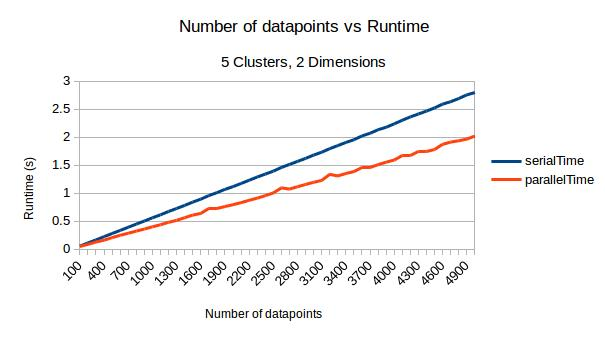
\includegraphics[width=0.9\linewidth, height=5cm]{Pictures/datapoints1.jpg}
        \caption{Serial vs. Parallel iterating datapoints, 5 clusters, 2 dimensions}
    \end{subfigure}
    \begin{subfigure}{0.5\textwidth}
        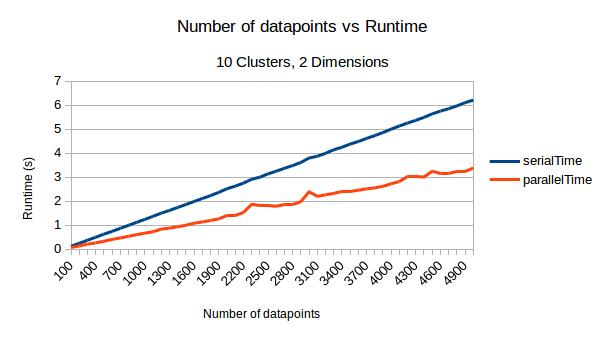
\includegraphics[width=0.9\linewidth, height=5cm]{Pictures/datapoints2.jpg}
        \caption{Serial vs. Parallel iterating datapoints, 10 clusters, 2 dimensions}
    \end{subfigure}
\caption{Graphs of results obtained iterating through the number of datapoints (100..5000, increments of 100)}
\end{figure}

Important to note is the difference between the two graphs. The graph of results using 10 clusters provides better speedup than the graph of results using 5 clusters. This portrays the idea of the multiple aspects we considered. We can expect to see healthy results when iterating through the number of clusters. In summary of these graphs, the serial algorithm doesn't change it's slope and more clusters makes it have a longer runtime. The parallel algorithm, however, does change it's slope when more clusters are used, becoming shallower and hence providing even better speedup for more clusters.

\newpage
\subsubsection{Serial vs Parallel Results (Iterating clusters)}
\begin{figure}[h!]
    \begin{subfigure}{0.5\textwidth}
        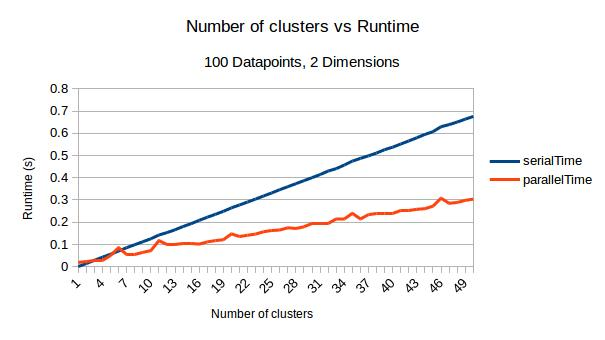
\includegraphics[width=0.9\linewidth, height=5cm]{Pictures/clusters1.jpg}
        \caption{Serial vs. Parallel iterating datapoints, 100 datapoints, 2 dimensions}
    \end{subfigure}
    \begin{subfigure}{0.5\textwidth}
        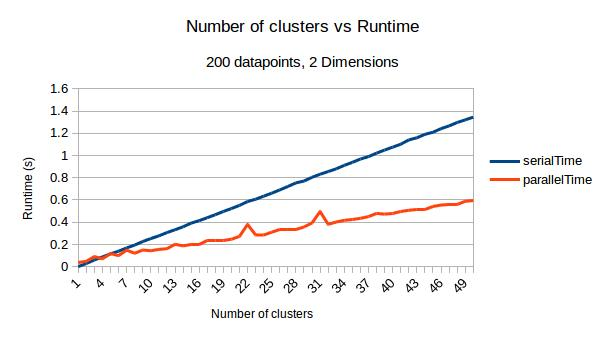
\includegraphics[width=0.9\linewidth, height=5cm]{Pictures/clusters2.jpg}
        \caption{Serial vs. Parallel iterating datapoints, 200 datapoints, 2 dimensions}
    \end{subfigure}
\caption{Graphs of results obtained iterating through the number of clusters (1..50, increments of 1)}
\end{figure}

Here we notice the graphs are not that different from eachother except in real terms. This is really to be expected as the number of datapoints used is very small. If we look back at the graphs of serial vs. parallel iterating through datapoints in section 9.1.1, the 100 and 200 datapoints mark doesn't provide substantial difference. This implies that the speedup in the cluster parallelization aspect in these results are more pure and unaffected by the gains of the datapoints parallelization. If we ran tests for higher numbers of data points we would see the orange line obtaining a shallower gradient (ie better speedup for more datapoints) due to the effects of iterations through datapoints being parallelized. Such tests were not ran as the time taken to run them is exorbitant.

\newpage
\subsection{Speedup Results}
\subsubsection{Serial vs Parallel Speedup Results (Iterating datapoints)}
\begin{figure}[h!]
    \begin{subfigure}{0.5\textwidth}
        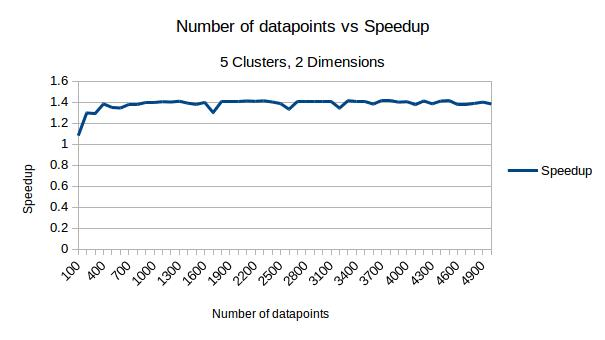
\includegraphics[width=0.9\linewidth, height=5cm]{Pictures/datapoints1_Speedup.jpg}
        \caption{Serial vs. Parallel iterating datapoints, 5 clusters, 2 dimensions}
    \end{subfigure}
    \begin{subfigure}{0.5\textwidth}
        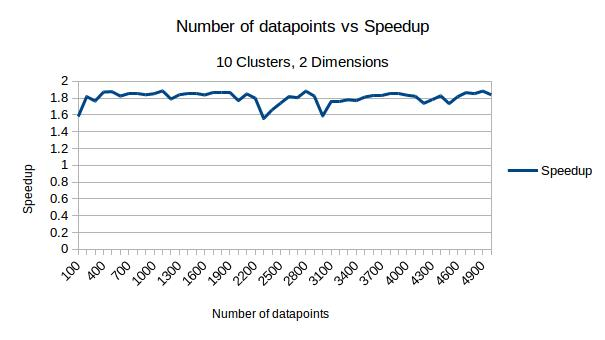
\includegraphics[width=0.9\linewidth, height=5cm]{Pictures/datapoints2_Speedup.jpg}
        \caption{Serial vs. Parallel iterating datapoints, 10 clusters, 2 dimensions}
    \end{subfigure}
\caption{Graphs of results obtained iterating through the number of datapoints (100..5000, increments of 100)}
\end{figure}

Here we see the same approximate shape between the two graphs. The second graph (using 10 clusters) has a higher speedup than the first. This is expected as we discussed the second graph in section 9.1.1 providing better speedup for more clusters. This is merely outlined by these two graphs. 

\newpage
\subsubsection{Serial vs Parallel Speedup Results (Iterating clusters)}
\begin{figure}[h!]
    \begin{subfigure}{0.5\textwidth}
        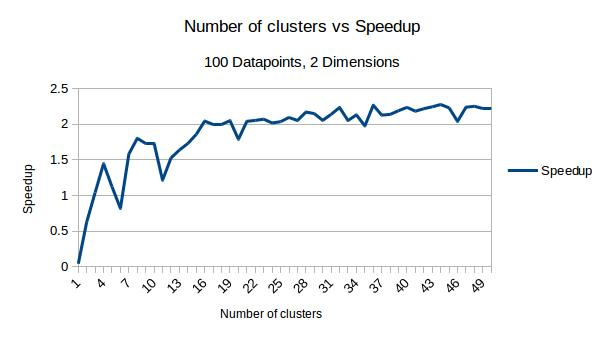
\includegraphics[width=0.9\linewidth, height=5cm]{Pictures/clusters1_Speedup.jpg}
        \caption{Serial vs. Parallel iterating datapoints, 100 datapoints, 2 dimensions}
    \end{subfigure}
    \begin{subfigure}{0.5\textwidth}
        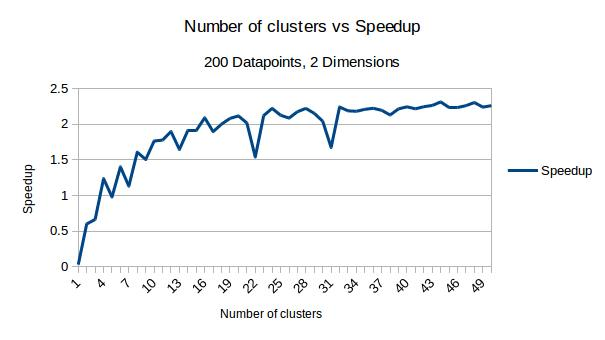
\includegraphics[width=0.9\linewidth, height=5cm]{Pictures/clusters2_Speedup.jpg}
        \caption{Serial vs. Parallel iterating datapoints, 200 datapoints, 2 dimensions}
    \end{subfigure}
\caption{Graphs of results obtained iterating through the number of clusters (1..50, increments of 1)}
\end{figure}

Here we see very similar graphs as again, as mentioned in section 9.1.2, the difference between 100 and 200 datapoints does not provide substantial gains. What is interesting, however, is the fact that these two graphs take a while before reaching optimal speedup. At around 15 clusters, the speedup breaks the 2.0x mark. The speed up does increase slightly past this however it is important to note that speedup is in fact below 1.0x up to about 5 clusters, which then sees a 1.0x speedup. This is important because it depicts the overhead of the parallelization outweighing the gains when fewer than 5 clusters are used. Code can be added to obtain a flat 1.0x speedup for fewer than 5 clusters.

\section{Conclusion}
In conclusion, the project was successful as we obtained respectable speedup for our algorithm. It is noteworthy that cluster parallelization provides better speedup than datapoint parallelization. This is likely due to the parallelization of random cluster generation, an infamously time consuming operation.

However, it is also important to note that while cluster speedup is higher than datapoint speedup, the datapoint speedup is very important as it is the aspect that is most likely to be increased in size.




\end{document}
